%%%%%%%%%%%%%%%%%%%%%%%%%%%%%%%%%%%%%%%%%%%%%%%%%%%%%%%%%%%%%%%%%%%%%%
% writeLaTeX Example: A quick guide to LaTeX
%
% Source: Dave Richeson (divisbyzero.com), Dickinson College
% 
% A one-size-fits-all LaTeX cheat sheet. Kept to two pages, so it 
% can be printed (double-sided) on one piece of paper
% 
% Feel free to distribute this example, but please keep the referral
% to divisbyzero.com
% 
%%%%%%%%%%%%%%%%%%%%%%%%%%%%%%%%%%%%%%%%%%%%%%%%%%%%%%%%%%%%%%%%%%%%%%
% How to use writeLaTeX: 
%
% You edit the source code here on the left, and the preview on the
% right shows you the result within a few seconds.
%
% Bookmark this page and share the URL with your co-authors. They can
% edit at the same time!
%
% You can upload figures, bibliographies, custom classes and
% styles using the files menu.
%
% If you're new to LaTeX, the wikibook is a great place to start:
% http://en.wikibooks.org/wiki/LaTeX
%
%%%%%%%%%%%%%%%%%%%%%%%%%%%%%%%%%%%%%%%%%%%%%%%%%%%%%%%%%%%%%%%%%%%%%%

\documentclass[10pt,UTF8,a4paper]{ctexart}
\usepackage{amssymb,amsmath,amsthm,amsfonts}
\usepackage{multicol,multirow}
\usepackage{calc}
\usepackage{ifthen}
\usepackage[landscape]{geometry}
\usepackage{listings}
\usepackage{hyperref}
\usepackage{graphicx}
\usepackage{color}
\usepackage{xcolor}

\everymath{\displaystyle}
\setmainfont{Times New Roman}
\setmathrm{Times New Roman}

\usepackage[complete,subscriptcorrection,slantedGreek,nofontinfo,mtphrb,zswash,mtpcal]{mtpro2}
\usepackage{bm}


\hypersetup{colorlinks=true,
            linkcolor=black,
            anchorcolor=blue,
            citecolor=green
            }

\lstdefinestyle{lfonts}{
    basicstyle=\footnotesize\ttfamily,
    stringstyle=\color{purple},
    keywordstyle=\color{blue!60!black}\bfseries,
    commentstyle=\color{olive}\scshape,
}
\lstdefinestyle{lnumbers}{
    numbers=left,
    numberstyle=\tiny,
    numbersep=1em,
    firstnumber=1,
    stepnumber=1,
}
\lstdefinestyle{llayout}{
    breaklines=true,
    tabsize=4,
    columns=flexible,
}
\lstdefinestyle{lgeometrya}{
    xleftmargin=20pt,
    xrightmargin=0pt,
    frame=tb,
    framesep=\fboxsep,
    framexleftmargin=20pt,
}
\lstdefinestyle{lgeneral}{
    style=lfonts,
    style=lnumbers,
    style=llayout,
    style=lgeometrya,
}
\lstdefinestyle{python}{
    language={Python},
    style=lgeneral,
    %columns = fixed,
    frame = shadowbox,
    %backgroundcolor = \color{yellow!10},
    rulesepcolor= \color{gray}
}

\ifthenelse{\lengthtest { \paperwidth = 11in}}
    { \geometry{top=.5in,left=.5in,right=.5in,bottom=.5in} }
	{\ifthenelse{ \lengthtest{ \paperwidth = 297mm}}
		{\geometry{top=1cm,left=1cm,right=1cm,bottom=1cm} }
		{\geometry{top=1cm,left=1cm,right=1cm,bottom=1cm} }
	}
\pagestyle{empty}
\makeatletter
\renewcommand{\section}{\@startsection{section}{1}{0mm}%
                                {1ex plus -.5ex minus -.2ex}%
                                {0ex plus .2ex}%x
                                {\normalfont\large\bfseries}}
\renewcommand{\subsection}{\@startsection{subsection}{2}{0mm}%
                                {1ex plus -.5ex minus -.2ex}%
                                {0ex plus .2ex}%
                                {\normalfont\normalsize\bfseries}}
\renewcommand{\subsubsection}{\@startsection{subsubsection}{3}{0mm}%
                                {1ex plus -.5ex minus -.2ex}%
                                {0ex plus .2ex}%
                                {\normalfont\small\bfseries}}
\makeatother
\setcounter{secnumdepth}{2}
%\setlength{\parindent}{0pt}
%\setlength{\parskip}{0pt plus 0.5ex}
\linespread{1}
\setlength{\parskip}{0pt plus 0.5ex}
%\setlength\parindent{2em}

% -----------------------------------------------------------------------

\title{数据结构与算法B  Cheat Sheet}

\begin{document}

\raggedright
\footnotesize

\begin{center}
     \Large{\textbf{数据结构与算法B  Cheat Sheet}} \\
\end{center}
\begin{multicols}{3}
\setlength{\premulticols}{1pt}
\setlength{\postmulticols}{1pt}
\setlength{\multicolsep}{1pt}
\setlength{\columnsep}{2pt}
%\setlength\parindent{2em}

\section{绪论}
\subsection{算法的时间复杂度及其表示法}
\subsubsection{什么是算法}
算法是对计算过程的描述,是为了解决某个问题而设计的有限长操作序列。

\subsubsection{算法的性质}
\textbf{有穷性:}一个算法必须可以用有穷条指令描述,且必须在执行有穷次操作后终止。每次操作都必须在有穷时间内完成。算法终止后必须给出所处理问题的解或宣告问题无解。

\textbf{确定性:}一个算法,对于相同的输入,无论运行多少次,总是得到相同的输出。也可以说只要算法运行前的初始条件相同,那么算法运行的结果也相同。

\textbf{可行性:}算法中的指令(或描述语句)含义明确无歧义,且可以被机械化地自动执行。

\textbf{输入/输出:}输入指的是描述算法所处理的问题的数据,输出指的是描述该问题的答案的数据。算法可以不需要输入。但是没有输出的算法是没有意义的。

\subsubsection{程序或算法的时间复杂度}
一个程序或算法的时间效率,也称“时间复杂度”,有时简称“复杂度”。

复杂度常用大的字母$O$和小写字母$n$来表示,比如$O(n)$,$O(n^2)$等。$n$代表问题的规模,$O(X)$就表示解决问题的时间和$X$成正比关系(粗略理解)。


时间复杂度是用算法运行过程中,某种时间固定的操作需要被执行的次数和n的关系来度量的。在无序数列中查找某个数,复杂度是$O(n)$。


计算复杂度的时候,只统计执行次数最多的($n$足够大时)那种固定操作(称为基本操作)的次数。比如某个算法需要执行加法$n^2$次,除法$10000n$次,那么就记其复杂度是$O(n^2)$的。

如果复杂度是多个$n$的函数之和,则只关心随$n$的增长增长得最快的那个函数。

\subsubsection{程序或算法的时间复杂度}
在无序数列中查找某个数(顺序查找):$O(n)$

插入排序、选择排序等笨排序方法:$O(n^2)$

快速排序:$O(n\log(n))$

二分查找:$O(\log(n))$

\subsubsection{Python中一些操作的时间复杂度总结}
\textbf{$O(1)$复杂度的常见操作:}

1)根据下标访问列表、字符串、元组中的元素

2)在集合、字典中增删元素

3)调用列表的 \verb|append| 函数在列表末尾添加元素,以及用 \verb|pop()| 函数删除列表末尾元素

4)用 \verb|in| 判断元素是否在集合中或某关键字是否在字典中

5)以关键字为下标访问字典中的元素的值

6)用 \verb|len| 函数求列表、元组、集合、字典的元素个数

\textbf{$O(n)$复杂度的常见操作:}

1)用 \verb|in| 判断元素是否在字符串、元组、列表中

2)用 \verb|insert| 在列表中插入元素

3)用 \verb|remove| 或 \verb|del| 删除列表中的元素

4)用字符串、元组或列表的 \verb|find|、\verb|rfind|、\verb|index|等函数做顺序查找

5)用字符串、元组或列表的 \verb|count| 函数计算元素出现次数

6)用 \verb|max|, \verb|min|函数求列表、元组的最大值,最小值

7)列表和元组加法

\textbf{$O(n\log n)$复杂度的常见操作:}

Python自带排序 \verb|sort|, \verb|sorted|

\textbf{$O(\log n)$复杂度的常见操作:}

在排好序的列表或元组上进行二分查找(初始的查找区间是整个元组或列表,每次和查找区间中点比较大小,并缩小查找区间到原来的一半。类似于查英语词典)有序就会找得快!Pyhon并不自带二分查找函数。

\textbf{{\ttfamily in} 用于列表和用于字典、集合的区别}

\verb|a in b|

若 \verb|b| 是列表,字符串或元组,则该操作时间复杂度$O(n)$,即时间和 \verb|b| 的元素个数成正比

若 \verb|b| 是字典或集合,则该操作时间复杂度$O(1)$,即时间基本就是常数,和 \verb|b| 里元素个数无关

因此集合用于需要经常判断某个东西是不是在一堆东西里的情况

此种场合用列表替代集合,容易导致超时!!!!

\subsubsection{最坏复杂度、平均复杂度、最好复杂度}
算法的复杂度有最好情况下复杂度、最坏情况下的复杂度和平均复杂度之分,虽然许多情况下最坏复杂度和平均复杂度恰好相同。

快速排序为例,一般情况下待排序序列杂乱无章,这种情况下快速排序的复杂度就是平均复杂度$O(n\log(n))$,但是在待排序的序列处于基本有序或基本逆序的最坏情况下,其复杂度会变成$O(n^2)$。

\subsection{数据的逻辑结构和存储结构}
\subsubsection{什么是数据结构?}
数据结构(data structure)就是数据的组织和存储形式。描述一个数据结构,需要指出其逻辑结构、存储结构和可进行的操作。

将数据的单位称作“元素”或“结点”。数据结构描述的就是结点之间的关系。

\subsubsection{数据的逻辑结构}

从逻辑上描述结点之间的关系,和数据的存储方式无关。

\textbf{集合结构:}结点之间没有什么关系,只是属于同一集合。如 \verb|set|。

\textbf{线性结构:}除了最靠前的结点,每个结点有唯一前驱结点;除了最靠后的结点,每个结点有唯一后继结点。如 \verb|list|。

\textbf{树结构:}有且仅有一个结点称为”根结点”,其没有前驱(父结点);有若干个结点称为 “叶结点”,没有后继(子结点);其它结点有唯一前驱,有1个或多个后继。如家谱。

\textbf{图结构:}每个结点都可以有任意多个前驱和后继,两个结点还可以互为前驱后继。如铁路网,车站是结点。

\subsubsection{数据的存储结构}
数据在物理存储器上存储的方式,大部分情况下指的是数据在内存中存储的方式。

\textbf{顺序结构:}结点在内存中连续存放,所有结点占据一片连续的内存空间。如 \verb|list|。

\textbf{链接结构:}结点在内存中可不连续存放,每个结点中存有指针指向其前驱结点和/或后继结点。如链表,树。

\textbf{索引结构:}将结点的关键字信息(比如学生的学号)拿出来单独存储,并且为每个关键字 \verb|x| 配一个指针指向关键字为 \verb|x| 的结点,这样便于按照关键字查找到相应的结点。

\textbf{散列结构:}设置散列函数,散列函数以结点的关键字为参数,算出一个结点的存储位置。

\textbf{数据的逻辑结构和存储结构无关}

一种逻辑结构的数据,可以用不同的存储结构来存储。

树结构、图结构可以用链接结构存储,也可以用顺序结构存储。

线性结构可以用顺序结构存储,也可以用链接结构存储。

\subsubsection{数据结构上的操作}

\textbf{建立(初始化)}

\textbf{插入结点}

\textbf{删除结点}

\textbf{查找结点}

\textbf{求结点前驱或结点后继。}如线性表、树和图。

\textbf{随机访问。}即“找第 \verb|i| 个结点”,如顺序表。

掌握一个数据结构,不但要了解其逻辑结构、存储结构,以及其上进行的各种操作,还需要知道每种操作的时间复杂度。


\section{线性表}
\subsection{顺序表}
即Python的列表,以及其它语言中的数组

元素在内存中连续存放

每个元素都有唯一序号(下标),且根据序号访问(包括读取和修改)元素的时间复杂度是$O(1)$的  --- 随机访问

下标为 \verb|i| 的元素前驱下标为 \verb|i-1|,后继下标为 \verb|i+1|

    
\subsubsection{顺序表支持的操作}
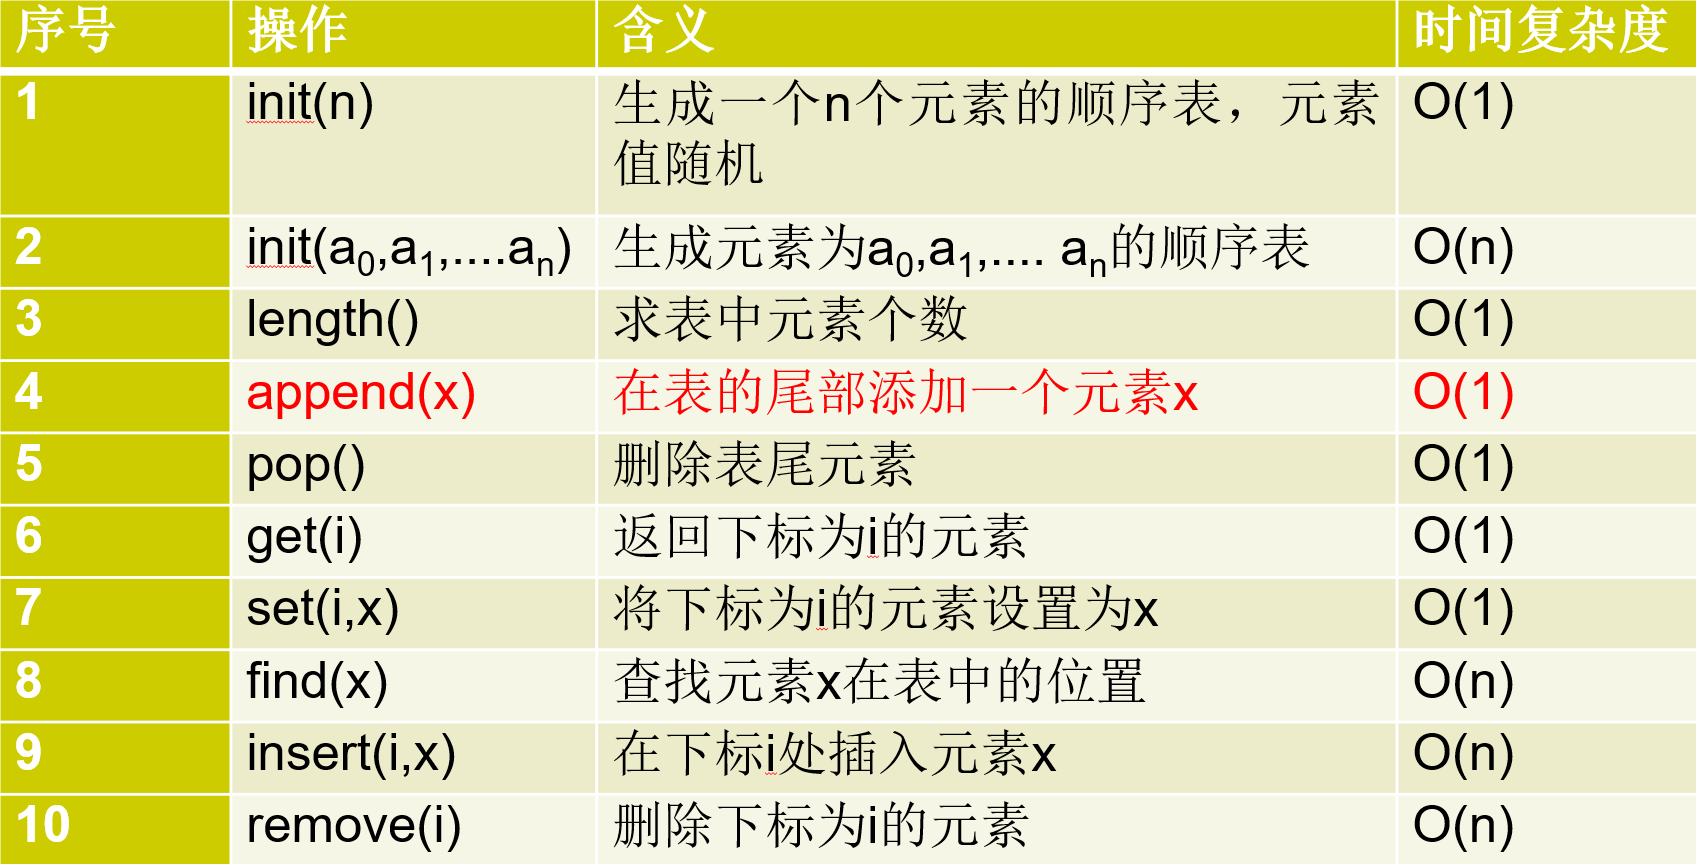
\includegraphics[width=\columnwidth]{images/顺序表支持的操作.png}

\subsubsection{顺序表的 {\ttfamily append} 的$O(1)$复杂度的实现}
总是分配多于实际元素个数的空间(容量大于元素个数)


元素个数小于容量时,\verb|append| 操作复杂度 $O(1)$


元素个数等于容量时,\verb|append| 导致重新分配空间,且要拷贝原有元素到新空间,复杂度 $O(n)$

重新分配空间时,新容量为旧容量的$k$倍($k>1$且固定),可确保 \verb|append| 操作的平均复杂度是$O(1)$。Python的 \verb|list| 取$k=1.2$左右。

\subsection{链表}
元素在内存中并非连续存放,元素之间通过指针链接起来

每个结点除了元素,还有 \verb|next| 指针,指向后继

不支持随机访问。访问第 \verb|i| 个元素,复杂度为$O(n)$

已经找到插入或删除位置的情况下,插入和删除元素的复杂度$O(1)$,且不需要复制或移动结点

有多种形式:单链表、循环单链表、双向链表、循环双向链表

\subsubsection{单链表}
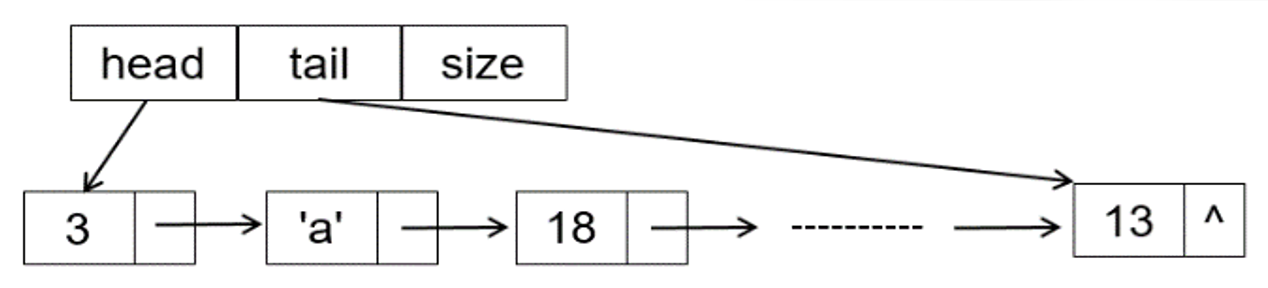
\includegraphics[width=\columnwidth]{images/单链表.png}
\begin{lstlisting}[style=python]
class LinkList:
	class Node: #表结点
		def __init__(self, data, next=None):
			self.data, self.next = data, next
	def __init__(self):
		self.head = self.tail = None
		self.size = 0

	def printList(self): #打印全部结点
		ptr = self.head
		while ptr is not None: 
			print(ptr.data, end=",")
			ptr = ptr.next

	def insert(self,p,data): #在结点p后面插入元素
		nd = LinkList.Node(data,None)
		if self.tail is p:  # 新增的结点是新表尾
			self.tail = nd
		nd.next = p.next
		p.next = nd
		self.size += 1
        
	def delete(self,p):  #删除p后面的结点
		if self.tail is p.next:
			self.tail = p
		p.next = p.next.next
		self.size -= 1

	#结点空间会被Python自动回收

\end{lstlisting}

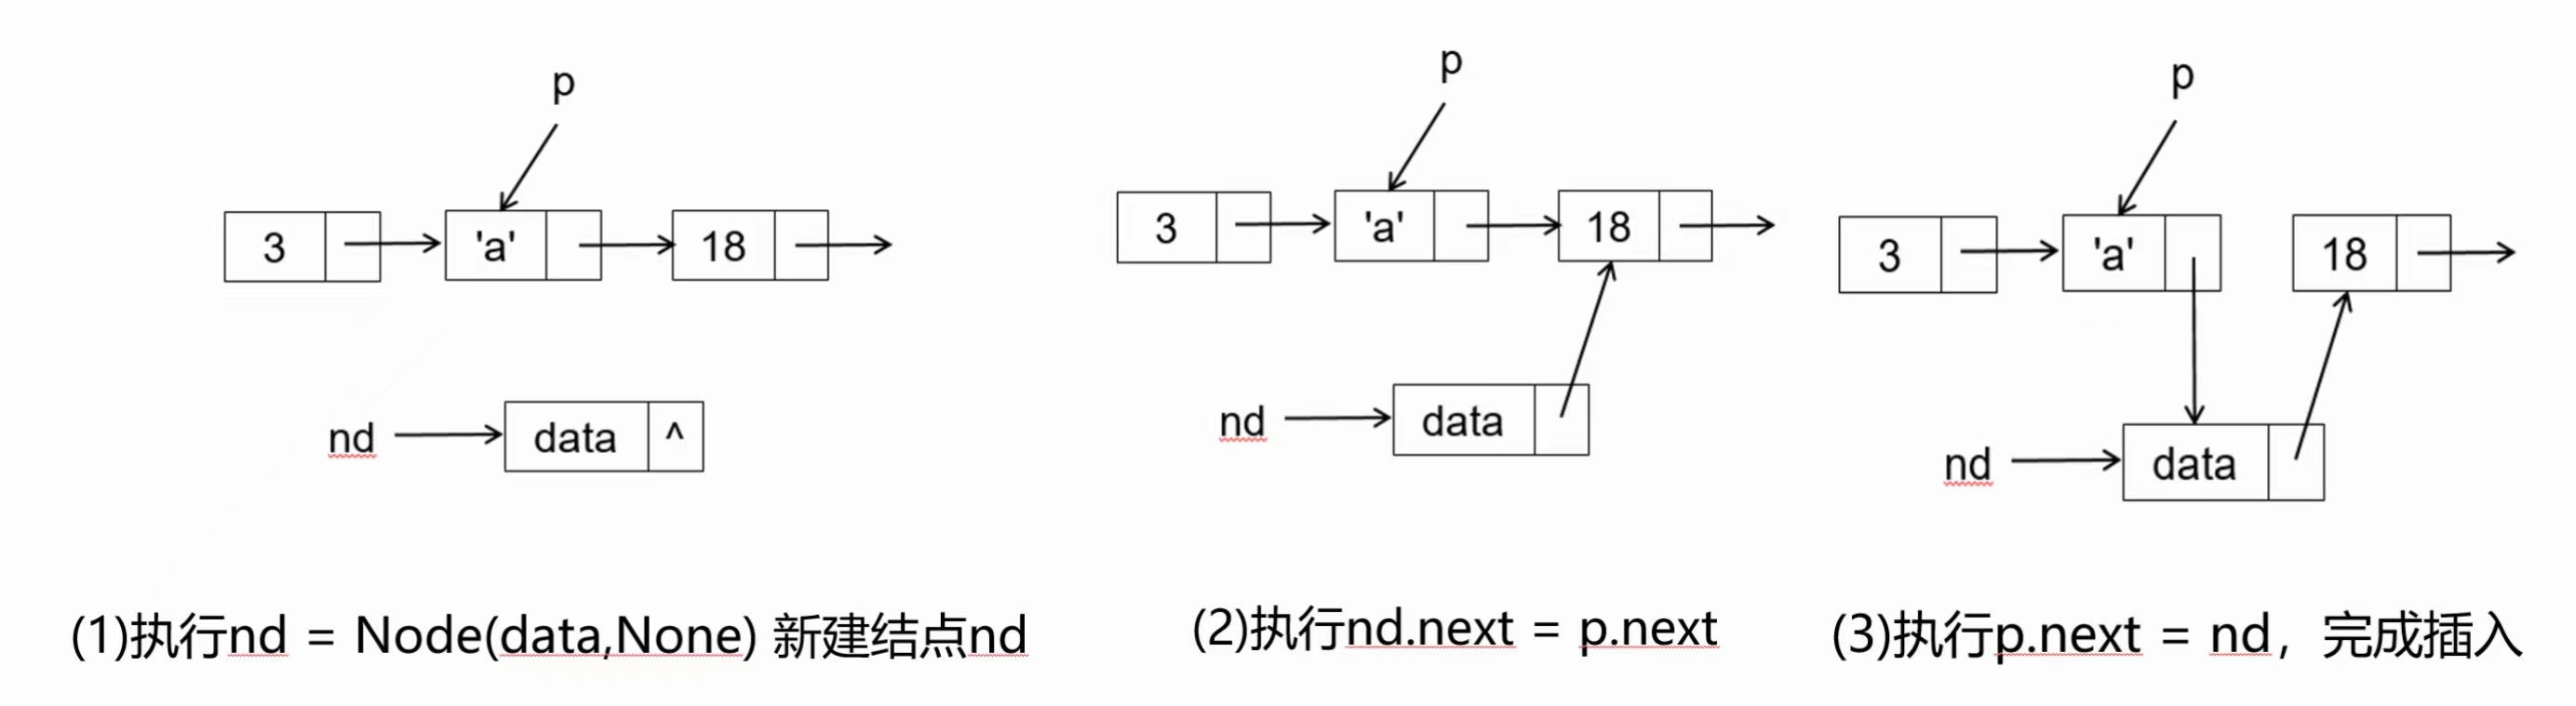
\includegraphics[width=\columnwidth]{images/单链表添加.jpg}

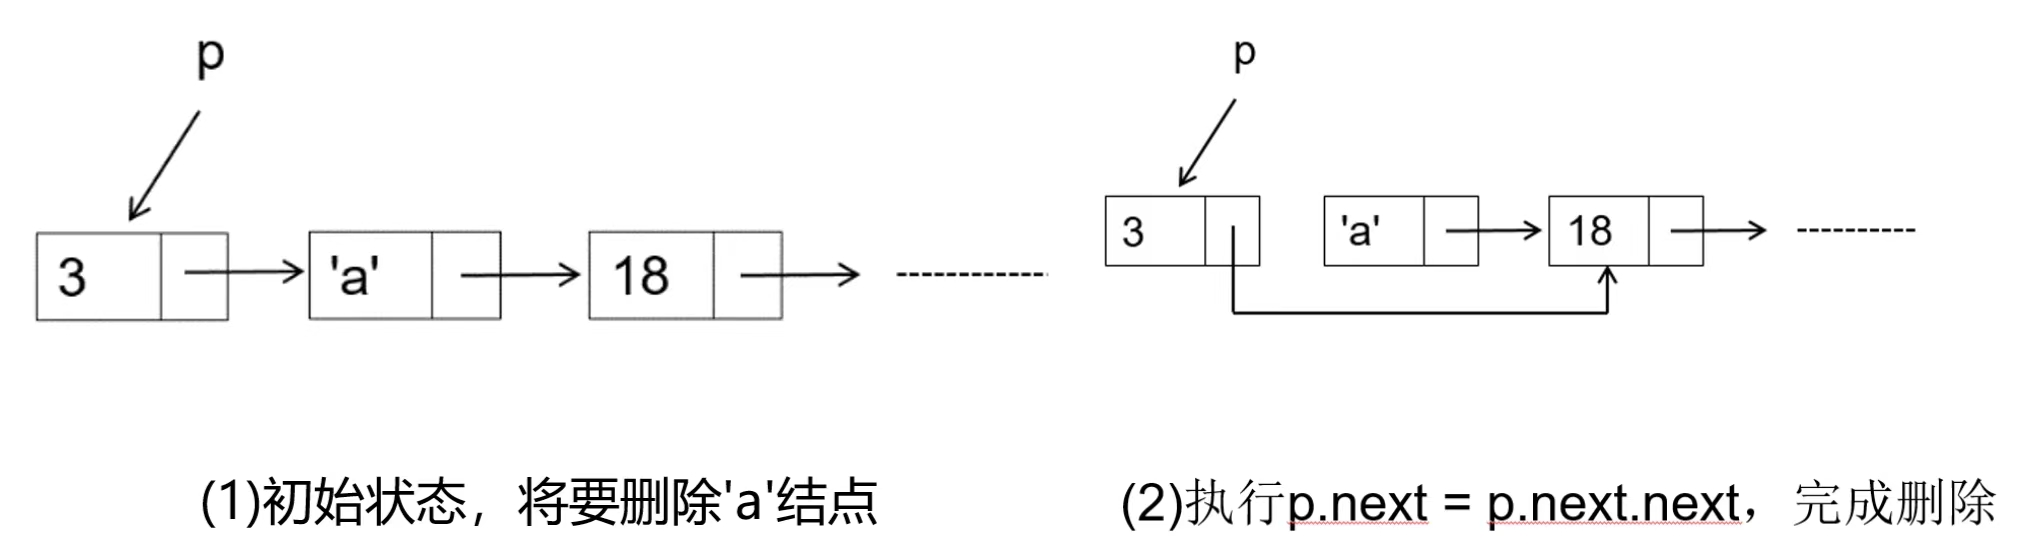
\includegraphics[width=\columnwidth]{images/单链表删除.jpg}

判断变量是否为 \verb|None|,应写 \verb|p is None, p is not None|
最好不要写 \verb|p == None, p != None|

\begin{lstlisting}[style=python]
	def popFront(self): #删除前端元素
		if self.head is None:
			raise \ 
		  Exception("Popping front for Empty link list.")
		else:
			self.head = self.head.next
			self.size -= 1
			if self.size == 0:
				self.head = self.tail = None
	def pushBack(self,data): #在尾部添加元素
		if self.size == 0:
			self.pushFront(data)
		else:
			self.insert(self.tail,data)

	def pushFront(self,data): #在链表前端插入一个元素data
		nd = LinkList.Node(data, self.head)
		self.head = nd
		self.size += 1
		if self.tail is None:
			self.tail = nd

	def clear(self):
		self.head = self.tail = None
		self.size = 0
	def __iter__(self):
		self.ptr = self.head
		return self
	def __next__(self):
		if self.ptr is None:
			raise StopIteration()  # 引发异常
		else:
			data = self.ptr.data
			self.ptr = self.ptr.next
			return data

\end{lstlisting}

\begin{lstlisting}[style=python]
linkLst = LinkList()
linkLst.pushFront(0)
linkLst.pushFront(1)
for i in range(2,5):
	linkLst.pushBack(i)
for x in linkLst:	#>>1,0,2,3,4,
	print(x,end=",")

\end{lstlisting}
上述实现方式没有实现“隐藏”,不是很好的实现方式

\subsubsection{带头结点的单链表}
为避免链表为空是做特殊处理,可以为链表增加一个空闲头结点

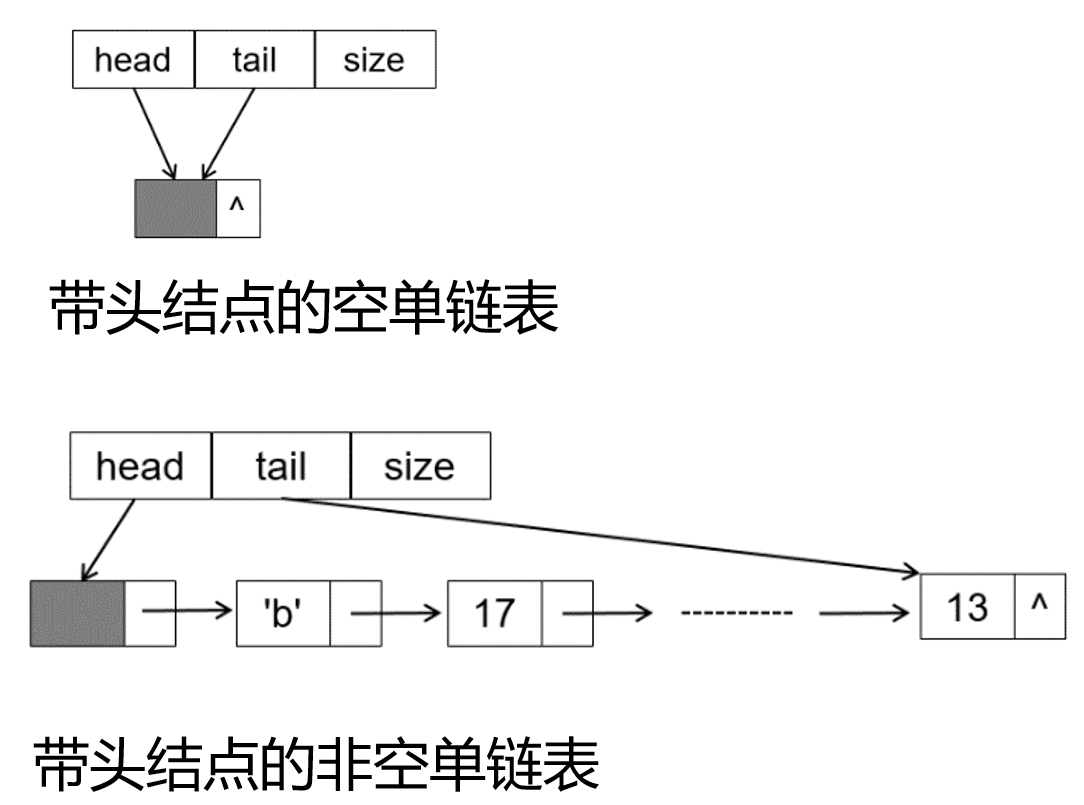
\includegraphics[width=.8\columnwidth]{images/头结点单链表.png}

\begin{lstlisting}[style=python]
class LinkList:
	def __init__(self):
		self.head = self.tail =  LinkList.Node(None,None)
		self.size = 0

\end{lstlisting}

\subsubsection{循环单链表}
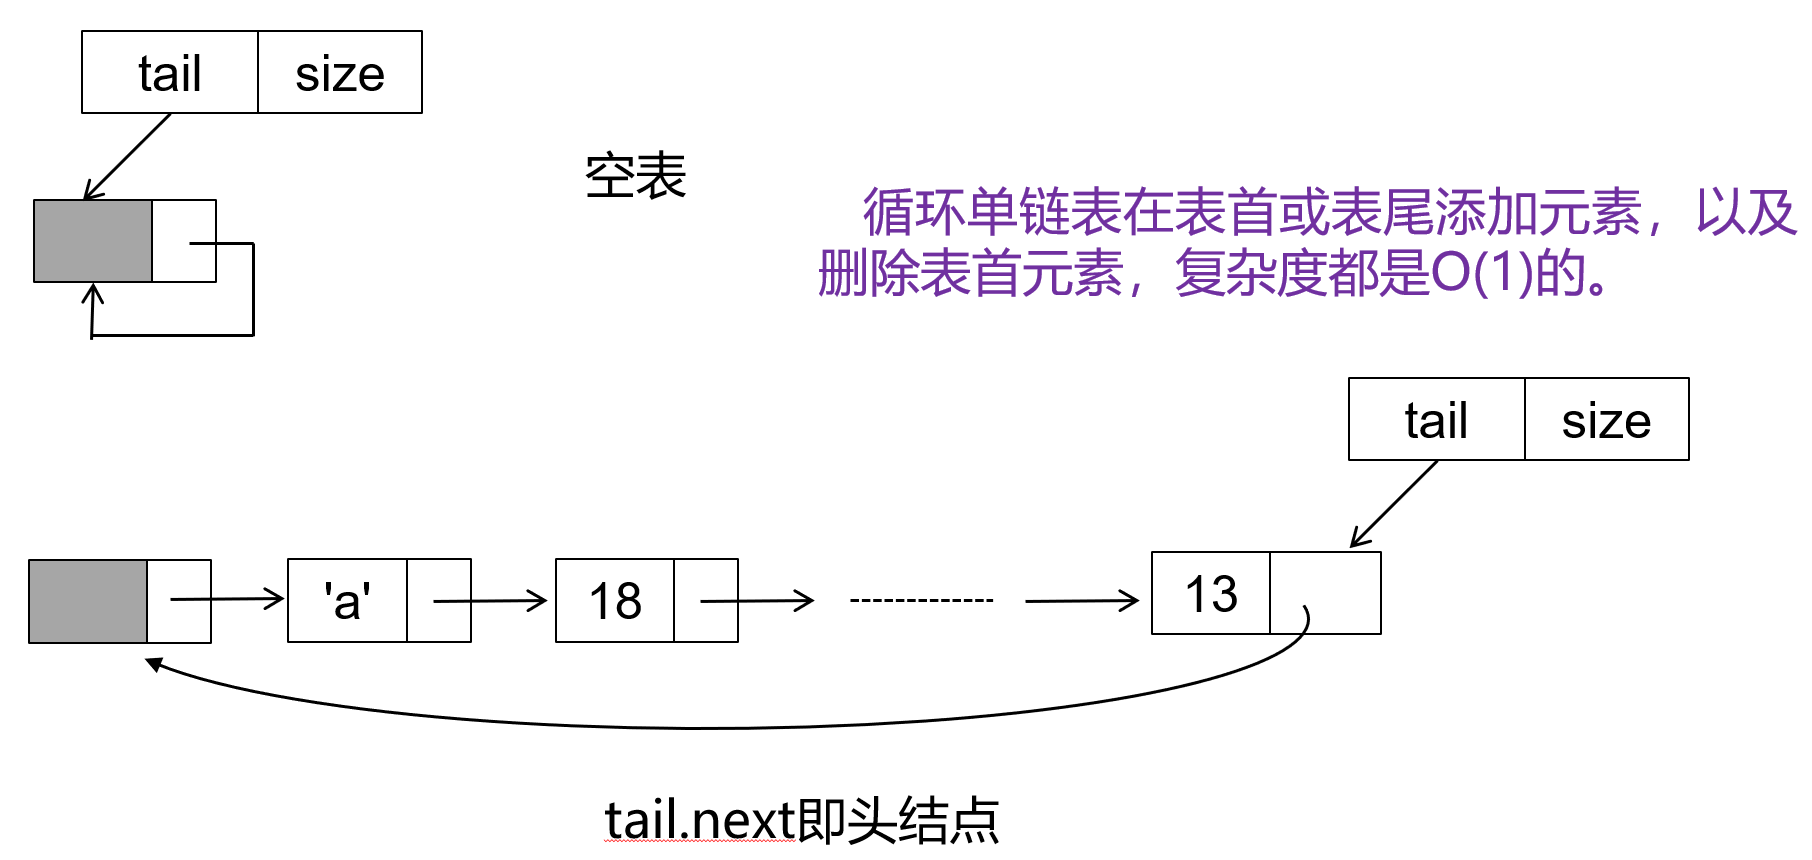
\includegraphics[width=\columnwidth]{images/循环单链表.png}

\subsubsection{双向链表}
每个结点有 \verb|text| 指针指向后继,有 \verb|prev| 指针指向前驱

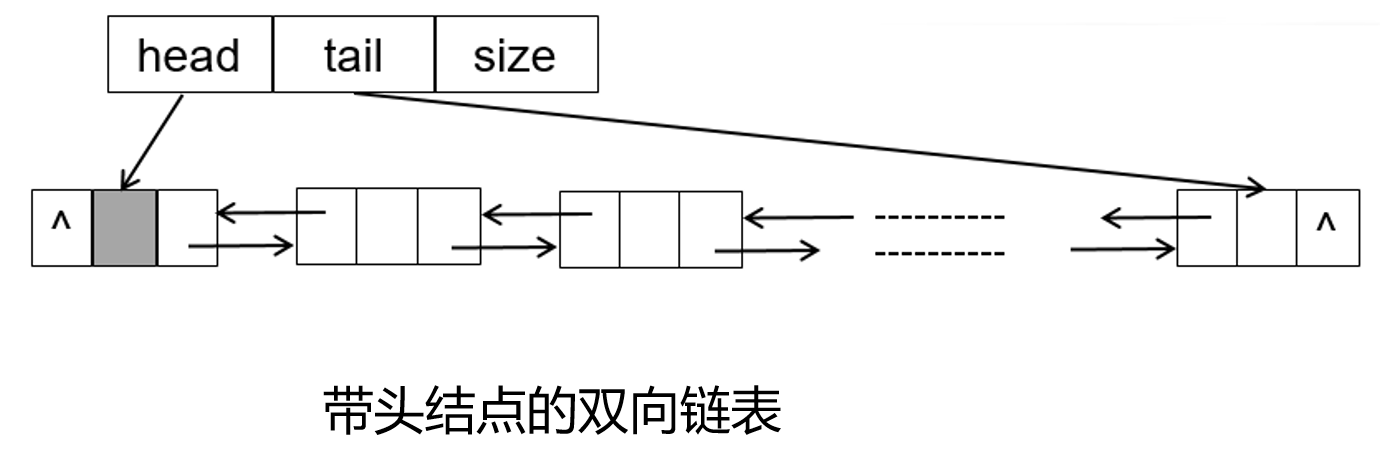
\includegraphics[width=\columnwidth]{images/带头结点的双向链表.png}

\begin{lstlisting}[style=python]
class DoubleLinkList:
	class _Node:
		def __init__(self, data, prev=None, next=None):
			self.data, self.prev, self.next = data, prev, next
\end{lstlisting}

在结点 \verb|p| 后面插入新结点 \verb|nd|

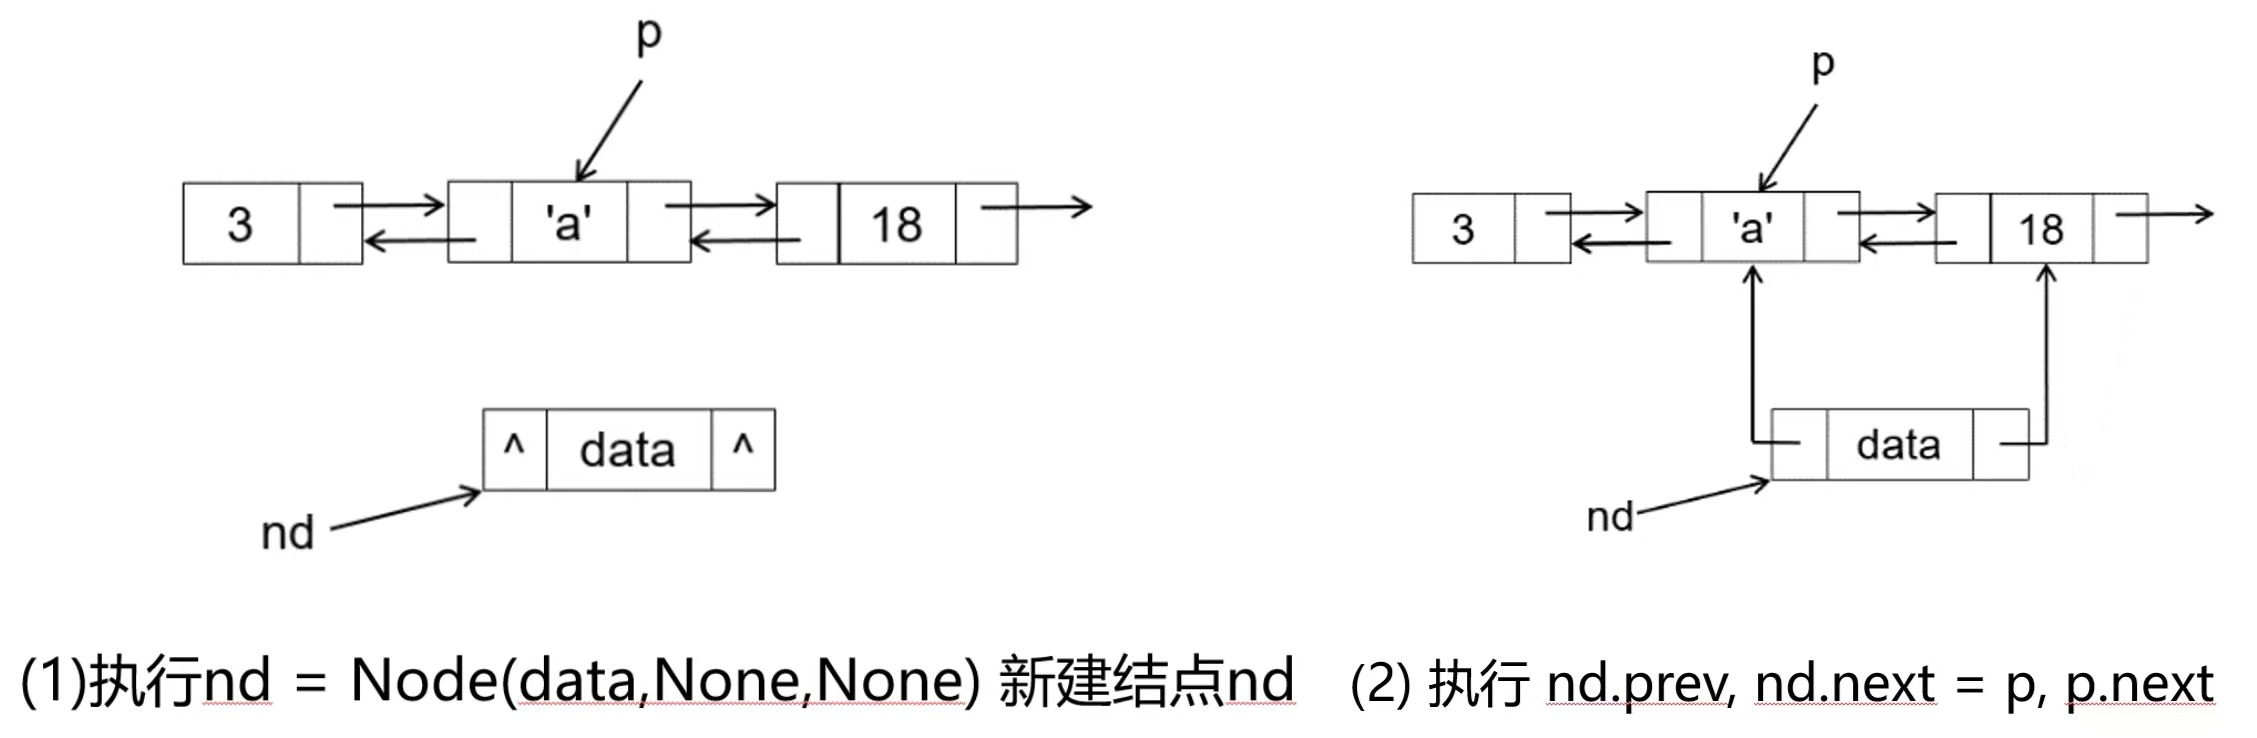
\includegraphics[width=\columnwidth]{images/双向链表插入1.jpg}
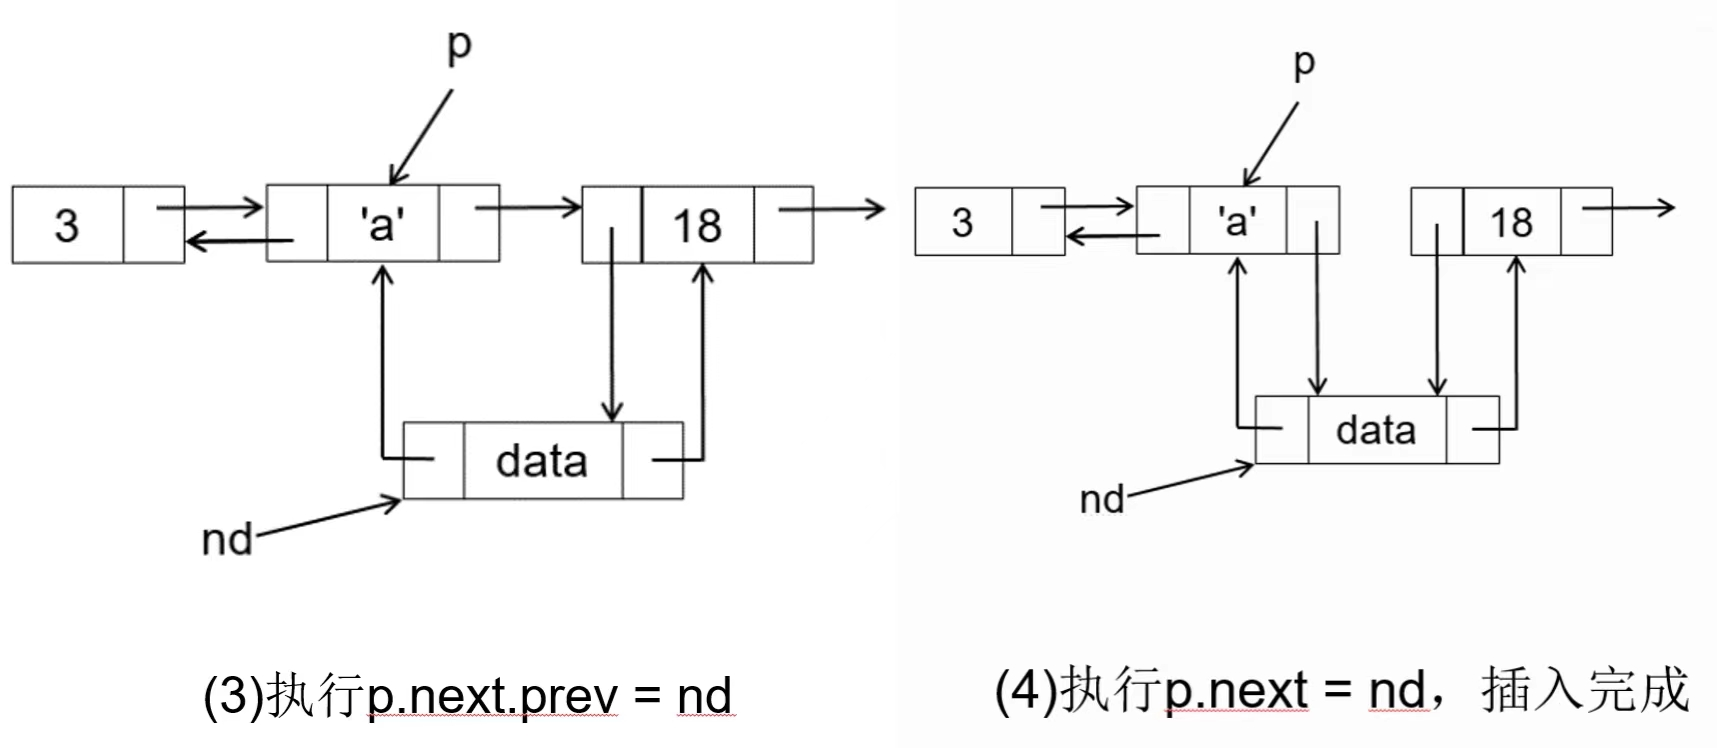
\includegraphics[width=\columnwidth]{images/双向链表插入2.jpg}

删除结点 \verb|p|

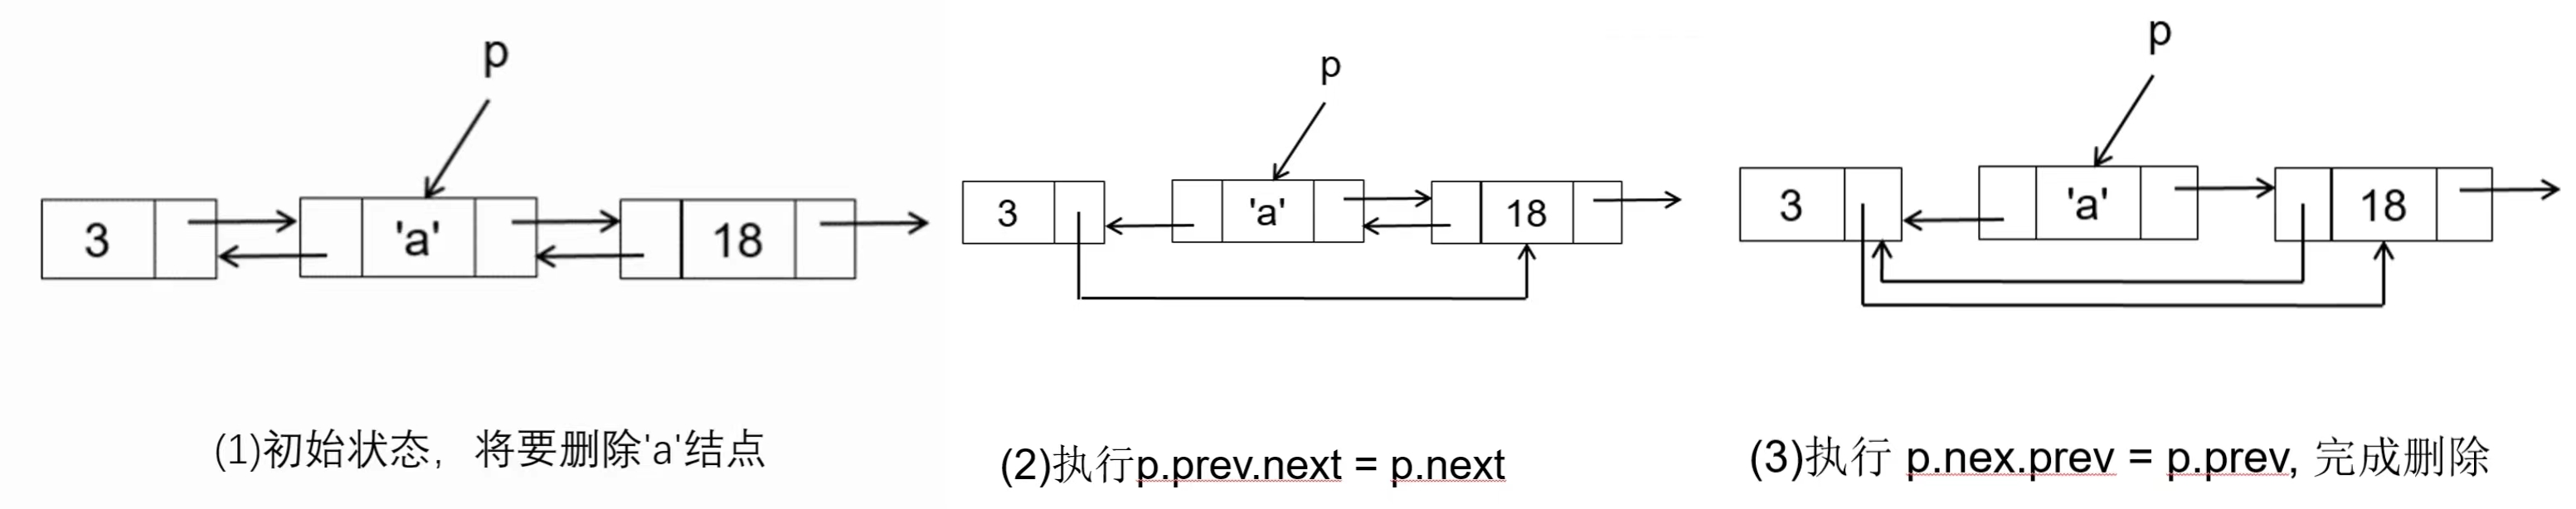
\includegraphics[width=\columnwidth]{images/双向链表删除.jpg}

双向链表实现
\begin{lstlisting}[style=python]
class DoubleLinkList:
	class _Node:
		def __init__(self, data, prev=None, next=None):
			self.data, self.prev, self.next = data, prev, next

	class _Iterator: 
		def __init__(self,p):
			self.ptr = p
		def getData(self):
			return self.ptr.data
		def setData(self,data):
			self.ptr.data = data
		def __next__(self):
			self.ptr = self.ptr.next
			if self.ptr is None:
				return None
			else:
				return DoubleLinkList._Iterator(self.ptr)
        def prev(self):
			self.ptr = self.ptr.prev
			return DoubleLinkList._Iterator(self.ptr)

	def __init__(self):
		self._head = self._tail = \
			DoubleLinkList._Node(None,None,None)
		self._size = 0

	def _insert(self,p,data):
		nd = DoubleLinkList._Node(data,p,p.next)
		if self._tail is p:  # 新增的结点是新表尾
			self._tail = nd
		if p.next:
			p.next.prev = nd
		p.next = nd
		self._size += 1

	def _delete(self,p):  #删除结点p
		if self._size == 0 or p is self._head:
			raise Exception("Illegal deleting.")
		else:
			p.prev.next = p.next
			if p.next: #如果p有后继
				p.next.prev = p.prev
			if self._tail is p:
				self._tail = p.prev
			self._size -= 1

	def clear(self):
		self._tail = self._head
		self._head.next = self._head.prev = None
		self.size = 0

	def begin(self):
		return DoubleLinkList._Iterator(self._head.next)

	def end(self):
		return None

	def insert(self,i,data): #在迭代器i指向的结点后面插入元素
		self._insert(i.ptr,data)

	def delete(self, i):  # 删除迭代器i指向的结点
		self._delete(i.ptr)

	def pushFront(self,data): #在链表前端插入一个元素
		self._insert(self._head,data)

	def popFront(self):
		self._delete(self._head.next)

	def pushBack(self,data):
		self._insert(self._tail,data)

	def popBack(self):
		self._delete(self._tail)

	def __iter__(self):
		self.ptr = self._head.next
		return self

	def __next__(self):
		if self.ptr is None:
			raise StopIteration()  # 引发异常
		else:
			data = self.ptr.data
			self.ptr = self.ptr.next
			return data

	def find(self,val): #查找元素val,找到返回迭代器,找不到返回None
		ptr = self._head.next
		while ptr is not None:
			if ptr.data == val:
				return DoubleLinkList._Iterator(ptr)
			ptr = ptr.next
		return self.end()

	def printList(self):
		ptr = self._head.next
		while ptr is not None:
			print(ptr.data,end=",")
			ptr = ptr.next

linkLst = DoubleLinkList()
for i in range(5):
	linkLst.pushBack(i)
i = linkLst.begin()
while i != linkLst.end(): #>>0,1,2,3,4,
	print(i.getData(),end = ",")
	i = next(i)
print()
i = linkLst.find(3)
i.setData(300)
linkLst.printList()  #>>0,1,2,300,4,
print()
linkLst.insert(i,6000) #在i后面插入6000
linkLst.printList() #>>0,1,2,300,6000,4,
print()
linkLst.delete(i)
linkLst.printList() #>>0,1,2,6000,4,


\end{lstlisting}

\subsection{链表和顺序表的选择}
\subsubsection{顺序表}
中间插入太慢

\subsubsection{链表}
访问第 \verb|i| 个元素太慢

顺序访问也慢(现代计算机有cache,访问连续内存域比跳着访问内存区域快很多)

还多费空间

\subsubsection{结论}
尽量选用顺序表。比如栈和队列,都没必要用链表实现

基本只有在找到一个位置后反复要在该位置周围进行增删,才适合用链表

实际工作中几乎用不到链表


\section{枚举与二分法}
\subsection{二分法寻找答案的核心思想}
如果一个假设的答案成立,那就跳着试一个更优的假设答案看行不行;

如果一个假设的答案不成立,那就跳着试一个更差的假设答案看行不行。

必须每次验证假设答案,都可以把假设答案所在的区间缩小为上次的一半。


前提:单调性。一个假设答案不成立,则比它更优的假设答案肯定都不成立。

\subsection{二分查找函数}
写一个函数 \verb|BinarySeach|,在从小到大排序的列表 \verb|a| 里查找元素 \verb|p|,如果找到,则返回元素下标,如果找不到,则返回 \verb|None|。要求复杂度$O(\log(n))$

\begin{lstlisting}[style=python]
def binarySearch(a,p,key = lambda x : x): 
    L, R = 0,len(a)-1  #查找区间的左右端点,区间含右端点 
    while L <= R: #如果查找区间不为空就继续查找 
        mid = L+(R-L)//2 #取查找区间正中元素的下标 
        if key(p) < key(a[mid]): 
            R = mid - 1  #设置新的查找区间的右端点 
        elif key(a[mid]) < key(p): 
            L = mid + 1  # 设置新的查找区间的左端点 
        else:
            return mid 
    return None
\end{lstlisting}

\section{递归和分治}
\subsection{递归}
\subsubsection{递归的作用}
1) 替代多重循环进行枚举

2) 解决本来就是用递归形式定义的问题

3) 将问题分解为规模更小的子问题进行求解

……

\section{栈和队列}
\subsection{栈}
类似于子弹匣,后压进去的子弹,先射出去

支持四种操作:

	\begin{tabular}{ll}
        \verb|top()|		&返回栈顶元素\\
        \verb|push(x)|		&将 \verb|x| 压入栈中\\
        \verb|pop()|		&弹出并返回栈顶元素\\
        \verb|isEmpty()|	&看栈是否为空
    \end{tabular}

要求上面操作复杂度都是$O(1)$

用列表可以实现栈

四种操作的实现(\verb|stack| 为一个列表):

	\begin{tabular}{ll}
        \verb|top()|		&\verb|stack[-1]|\\
        \verb|push(x)|		&\verb|stack.append(x)|\\
        \verb|pop()|		&\verb|stack.pop()|\\
        \verb|isEmpty()|	&\verb|len(stack) == 0|\\
    \end{tabular}

\subsection{队列}
即排队的队列。只能一头进(\verb|push|),另一头出(\verb|pop|)。先进先出

要求进出的复杂度都是$O(1)$

如果用列表的 \verb|append| 进,\verb|pop(0)| 出,则出的复杂度为$O(n)$

\subsubsection{队列的实现方法一}
用足够大的列表实现,维护一个队头指针和队尾指针,初始:\verb|head=tail = 0|

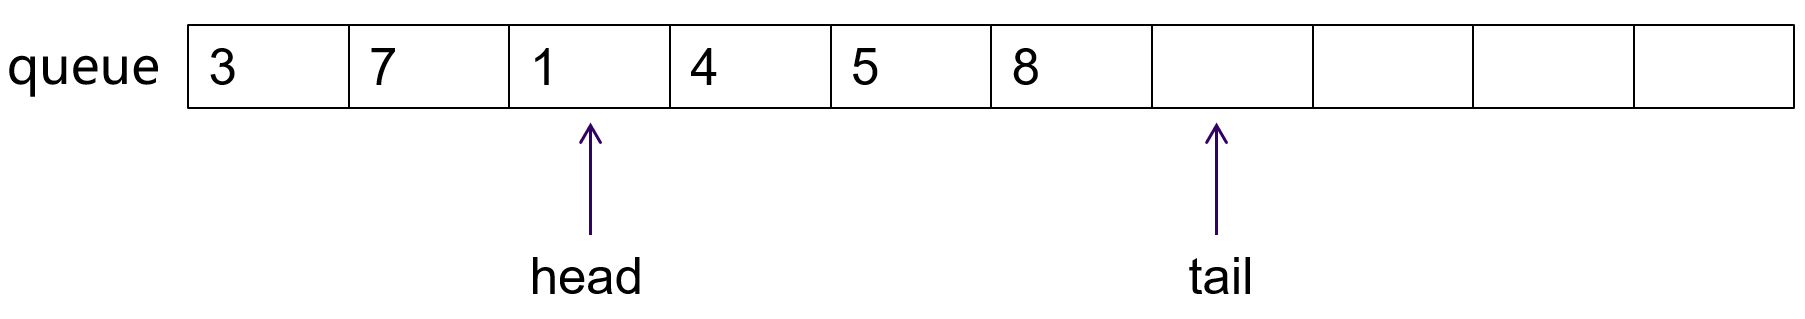
\includegraphics[width=\columnwidth]{images/队列1.png}

\verb|head| 指向队头元素,\verb|tail| 指向队尾元素的后面

\verb|push(x)| 的实现:

\verb|queue[tail] = x| 	

\verb|tail+=1|

\verb|pop()| 的实现:\verb|head += 1|

判断队列是否为空:\verb|head == tail|

\subsubsection{队列的实现方法二}
如果不想浪费空间开足够大的列表,而是想根据实际情况分配空间,则可以用列表+头尾循环法实现队列

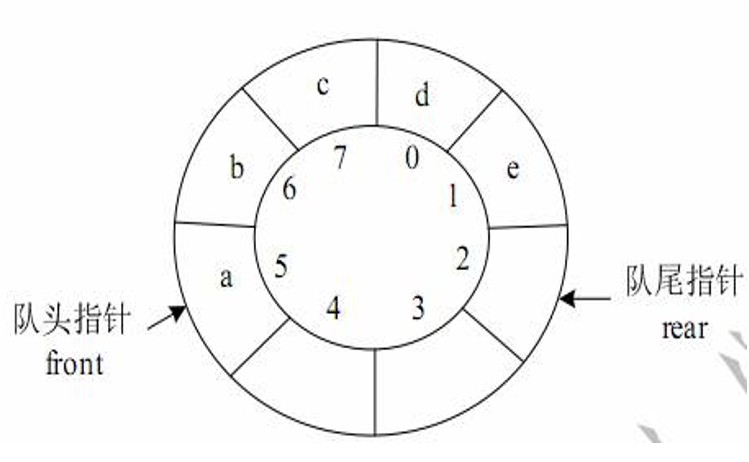
\includegraphics[width=\columnwidth]{images/队列2.png}

1) 预先开设一个 \verb|capacity| 个空元素的列表 \verb|queue|,\verb|head = tail = 0|

2) 列表没有装满的情况下:

\verb|push(x)| 的实现:

	\verb|queue[tail] = x|

	\verb|tail = (tail+1) % capacity|

\verb|pop()| 的实现:

	\verb|head =  (head+1) % capacity|

\verb|capacity| 可以是4,8,16.....

3) 如何判断队列是否为空:

    方法1:维护一个元素总数 \verb|size, size == 0| 即为空

    方法2:不维护 \verb|size|,浪费 \verb|queue| 中一个单元的存储空间

                 \verb|head == tail| 即为空

4) 如何判断队列是否为满:

    方法1:维护一个元素总数 \verb|size, size == capacity| 即为满

    方法2:不维护 \verb|size|, 浪费 \verb|queue| 中一个单元的存储空间,

	    \verb|(tail + 1) % capacity == head| 即为满

                 如果不浪费,就无法区分 \verb|head == tail| 是队列空导致,还是队列满导致


5) 若一个push操作后导致列表满:

i. 建一个大小是原列表$k$倍大的新列表($k>1$,可以取1.5,2.....)

ii. 将原列表内容全部拷贝到新列表,作为新队列

iii. 重新设置新列表的 \verb|head| 和 \verb|tail|   

iv. 原列表空间自动被Python解释器回收

导致队列满的 \verb|push| 的时间复杂度是$O(n)$。平均 \verb|push| 操作是 $O(1)$

Python列表 \verb|append| 做到$O(1)$的实现也是这种原理,且$k$取1.125,空间换时间

若每次增加空间只增加固定数量,比如20个单元,则 \verb|push| 平均复杂度还是$O(n)$

\begin{lstlisting}[style=python]
class Queue:
	_initC = 8		#存放队列的列表的初始容量
	_expandFactor = 1.5  #扩充容量时容量增加的倍数
	def __init__(self):
		self._q = [None for i in range(Queue._initC)]
		self._size = 0				    #队列元素个数
		self._capacity = Queue._initC #队列最大容量
		self._head = self._rear = 0
	def isEmpty(self):
		return self._size == 0
	def front(self):  #看队头元素。空队列导致re
		if self._size == 0:
			raise Exception("Queue is empty")
		return self._q[self._head]
	def back(self):   #看队尾元素,空队列导致re
		if self._size == 0:
			raise Exception("Queue is empty")
		if self._rear > 0:
			return self._q[self._rear - 1]
		else:
			return self._q[-1]
	def push(self,x):
		if self._size == self._capacity:
			tmp = [None for i in range(
					int(self._capacity*Queue._expandFactor))]
			k = 0
			while k < self._size:
				tmp[k] = self._q[self._head]
				self._head = (self._head + 1) % self._capacity
				k += 1
			self._q = tmp  #原来self._q的空间会被Python自动释放
			self._q[k] = x
			self._head,self._rear = 0,k+1
			self._capacity = int(
					self._capacity*Queue._expandFactor)
		else:
			self._q[self._rear] = x
			self._rear = (self._rear + 1) % self._capacity
		self._size += 1
	def pop(self):
		if self._size == 0:
			raise Exception("Queue is empty")
		self._size -= 1
		self._head = (self._head + 1) % len(self._q)

q = Queue()
for i in range(1,314):
	q.push(i)
	print(q.back(),end=",")
print()
while not q.isEmpty():
	print(q.front(),end=",")
	q.pop()


\end{lstlisting}

\subsubsection{用两个栈实现一个队列}


执行 \verb|push(x)| 操作时,将 \verb|x| 压入栈 \verb|inStack|,执行 \verb|pop()| 或 \verb|front()| 操作时,看另一个栈 \verb|outStack| 是否为空,若不为空,弹出栈顶元素或访问栈顶元素即可;若为空,则先将 \verb|inStack| 中的全部元素弹出并依次压入 \verb|outStack|,然后再弹出或访问 \verb|outStack| 的栈顶元素。



由于每个元素最多出入 \verb|inStack| 各一次,出入 \verb|outStack| 各一次,所以 \verb|pop| 和 \verb|front| 操作的平均复杂度是 $O(1)$的。

























\section{Math vs. text vs. functions}
In properly typeset mathematics  variables appear in italics (e.g., $f(x)=x^{2}+2x-3$). The exception to this rule is predefined functions (e.g., $\sin (x)$). Thus it is important to \textbf{always} treat text, variables, and functions correctly. See the difference between $x$ and x, -1 and $-1$, and $sin(x)$ and $\sin(x)$.  

There are two ways to present a mathematical expression--- \emph{inline} or as an \emph{equation}.

\subsection{Inline mathematical expressions}
Inline expressions occur in the middle of a sentence.  To produce an inline expression, place the math expression between dollar signs (\verb!$!).  For example, typing \verb!$90^{\circ}$ is the same as $\frac{\pi}{2}$ radians!  yields $90^{\circ}$ is the same as $\frac{\pi}{2}$ radians.

\subsection{Equations}
Equations are mathematical expressions that are given their own line and are centered on the page.  These are usually used for important equations that deserve to be showcased on their own line or for large equations that cannot fit inline. To produce an inline expression, place the mathematical expression  between the symbols  \verb!\[! and \verb!\]!. Typing \verb!\[x=\frac{-b\pm\sqrt{b^2-4ac}}{2a}\]! yields \[x=\frac{-b\pm\sqrt{b^2-4ac}}{2a}.\]
 
\subsection{Displaystyle} 
To get full-sized inline mathematical expressions  use  \verb!\displaystyle!. Use this sparingly. Typing \verb!I want this $\displaystyle \sum_{n=1}^{\infty}! \verb!\frac{1}{n}$, not this $\sum_{n=1}^{\infty}! \verb!\frac{1}{n}$.! yields\\ I want  this $\displaystyle \sum_{n=1}^{\infty}\frac{1}{n}$, not this $\sum_{n=1}^{\infty}\frac{1}{n}.$


\section{Images}

You can put images (pdf, png, jpg, or gif) in your document. They need to be in the same location as your .tex file when you compile the document. Omit   \verb![width=.5in]! if you want the image to be full-sized.

\verb!\begin{figure}[ht]!\\
\verb!\includegraphics[width=.5in]{imagename.jpg}!\\
\verb!\caption{The (optional) caption goes here.}!\\
\verb!\end{figure}!

\subsection{Text decorations}

Your text can be \textit{italics} (\verb!\textit{italics}!), \textbf{boldface} (\verb!\textbf{boldface}!), or \underline{underlined} (\verb!\underline{underlined}!).

Your math can contain boldface, $\mathbf{R}$ (\verb!\mathbf{R}!), or blackboard bold, $\mathbb{R}$ (\verb!\mathbb{R}!). You may want to used these to express the sets of real numbers ($\mathbb{R}$ or $\mathbf{R}$), integers ($\mathbb{Z}$ or $\mathbf{Z}$), rational numbers ($\mathbb{Q}$ or $\mathbf{Q}$), and natural numbers ($\mathbb{N}$ or $\mathbf{N}$).

To have text appear in a math expression use \verb!\text!. \verb!(0,1]=\{x\in\mathbb{R}:x>0\text{ and }x\le 1\}! yields $(0,1]=\{x\in\mathbb{R}:x>0\text{ and }x\le 1\}$. (Without the \verb!\text! command it treats ``and'' as three variables: $(0,1]=\{x\in\mathbb{R}:x>0 and x\le 1\}$.)



\section{Spaces and new lines}

\LaTeX\ ignores extra spaces and new lines. For example, 

\verb!This   sentence will       look!

\verb!fine after      it is     compiled.!

This   sentence will       look
fine after      it is     compiled.


Leave one full empty line between two paragraphs. Place \verb!\\! at the end of a line to create a new line (but not create a new paragraph).

\verb!This!

\verb!compiles!

~

\verb!like\\!

\verb!this.!

This
compiles 

like\\
this.

Use  \verb!\noindent! to prevent a paragraph from indenting.

\section{Comments}

Use \verb!%! to create a comment. Nothing on the line after the \verb!%! will be typeset. \verb!$f(x)=\sin(x)$ %this is the sine function! yields $f(x)=\sin(x)$%this is the sine function

\section{Delimiters}

\begin{tabular}{lll}
\emph{description} & \emph{command} & \emph{output}\\
parentheses &\verb!(x)! & (x)\\
brackets &\verb![x]! & [x]\\
curly braces& \verb!\{x\}! & \{x\}\\
\end{tabular}

To make your delimiters large enough to fit the content, use them together with \verb!\right! and \verb!\left!. For example, \verb!\left\{\sin\left(\frac{1}{n}\right)\right\}_{n}^! \verb!{\infty}! produces\\ $\displaystyle \left\{\sin\left(\frac{1}{n}\right)\right\}_{n}^{\infty}$.

Curly braces are non-printing characters that are used to gather text that has more than one character. Observe the differences between the four expressions \verb!x^2!, \verb!x^{2}!, \verb!x^2t!, \verb!x^{2t}! when typeset: $x^2$, $x^{2}$, $x^2t$, $x^{2t}$.


\section{Lists}

You can produce ordered and unordered lists.

\begin{tabular}{lll}
\emph{description} & \emph{command} & \emph{output}\\
unordered list&
\begin{tabular}{l}
\verb!\begin{itemize}!\\
\verb!  \item!\\
\verb!  Thing 1!\\
\verb!  \item!\\
\verb!  Thing 2!\\
\verb!\end{itemize}!
\end{tabular}&
\begin{tabular}{l}
$\bullet$ Thing 1\\
$\bullet$ Thing 2
\end{tabular}\\
~\\
ordered list&
\begin{tabular}{l}
\verb!\begin{enumerate}!\\
\verb!  \item!\\
\verb!  Thing 1!\\
\verb!  \item!\\
\verb!  Thing 2!\\
\verb!\end{enumerate}!
\end{tabular}&
\begin{tabular}{l}
1.~Thing 1\\
2.~Thing 2
\end{tabular}
\end{tabular}


\section{Symbols (in \emph{math} mode)}

\subsection{The basics}
\begin{tabular}{lll}
\emph{description} & \emph{command} & \emph{output}\\
addition & \verb!+! & $+$\\
subtraction & \verb!-! & $-$\\
plus or minus & \verb!\pm! & $\pm$\\
multiplication (times) & \verb!\times! & $\times$\\
multiplication (dot) & \verb!\cdot! & $\cdot$\\
division symbol & \verb!\div! & $\div$\\
division (slash) & \verb!/! & $/$\\
circle plus & \verb!\oplus! & $\oplus$\\
circle times & \verb!\otimes! & $\otimes$\\
equal & \verb!=! & $=$\\
not equal & \verb!\ne! & $\ne$\\
less than & \verb!<! & $<$\\
greater than & \verb!>! & $>$\\
less than or equal to & \verb!\le! & $\le$\\
greater than or equal to & \verb!\ge! & $\ge$\\
approximately equal to & \verb!\approx! & $\approx$\\
infinity & \verb!\infty! & $\infty$\\
dots & \verb!1,2,3,\ldots! & $1,2,3,\ldots$\\
dots & \verb!1+2+3+\cdots! & $1+2+3+\cdots$\\
fraction & \verb!\frac{a}{b}! & $\frac{a}{b}$\\
square root & \verb!\sqrt{x}! & $\sqrt{x}$\\
$n$th root & \verb!\sqrt[n]{x}! & $\sqrt[n]{x}$\\
exponentiation & \verb!a^b! & $a^{b}$\\
subscript & \verb!a_b! & $a_{b}$\\
absolute value & \verb!|x|! & $|x|$\\
natural log  & \verb!\ln(x)! & $\ln(x)$\\
logarithms & \verb!\log_{a}b! & $\log_{a}b$\\
exponential function & \verb!e^x=\exp(x)! & $e^{x}=\exp(x)$\\
degree & \verb!\deg(f)! & $\deg(f)$\\
\end{tabular}

\subsection{Functions}
\begin{tabular}{lll}
\emph{description} & \emph{command} & \emph{output}\\
maps to & \verb!\to! & $\to$\\
composition& \verb!\circ! & $\circ$\\
piecewise& \verb!|x|=! & \multirow{5}{*}{$\displaystyle |x|=\begin{cases}x&x\ge 0\\-x&x<0\end{cases}$}\\
function&\verb!\begin{cases}!&\\ 
&\verb!x & x\ge 0\\!&\\ 
&\verb!-x & x<0!&\\ 
&\verb!\end{cases}!&
\end{tabular}

\subsection{Greek and Hebrew letters}
\begin{tabular}{llll}
\emph{command} & \emph{output}&\emph{command} & \emph{output}\\
\verb!\alpha! & $\alpha$&\verb!\tau! & $\tau$\\
\verb!\beta! & $\beta$&\verb!\theta! & $\theta$\\
\verb!\chi! & $\chi$&\verb!\upsilon! & $\upsilon$\\
\verb!\delta! & $\delta$&\verb!\xi! & $\xi$\\
\verb!\epsilon! & $\epsilon$&\verb!\zeta! & $\zeta$\\
\verb!\varepsilon! & $\varepsilon$&\verb!\Delta! & $\Delta$\\
\verb!\eta! & $\eta$&\verb!\Gamma! & $\Gamma$\\
\verb!\gamma! & $\gamma$&\verb!\Lambda! & $\Lambda$\\
\verb!\iota! & $\iota$&\verb!\Omega! & $\Omega$\\
\verb!\kappa! & $\kappa$&\verb!\Phi! & $\Phi$\\
\verb!\lambda! & $\lambda$&\verb!\Pi! & $\Pi$\\
\verb!\mu! & $\mu$&\verb!\Psi! & $\Psi$\\
\verb!\nu! & $\nu$&\verb!\Sigma! & $\Sigma$\\
\verb!\omega! & $\omega$&\verb!\Theta! & $\Theta$\\
\verb!\phi! & $\phi$&\verb!\Upsilon! & $\Upsilon$\\
\verb!\varphi! & $\varphi$&\verb!\Xi! & $\Xi$\\
\verb!\pi! & $\pi$&\verb!\aleph! & $\aleph$\\
\verb!\psi! & $\psi$&\verb!\beth! & $\beth$\\
\verb!\rho! & $\rho$&\verb!\daleth! & $\daleth$\\
\verb!\sigma! & $\sigma$&\verb!\gimel! & $\gimel$
\end{tabular}


\subsection{Set theory}
\begin{tabular}{lll}
\emph{description} & \emph{command} & \emph{output}\\
set brackets & \verb!\{1,2,3\}! & $\{1,2,3\}$\\
element of & \verb!\in! & $\in$\\
not an element of & \verb!\not\in! & $\not\in$\\
subset of & \verb!\subset! & $\subset$\\
subset of & \verb!\subseteq! & $\subseteq$\\
not a subset of & \verb!\not\subset! & $\not\subset$\\
contains & \verb!\supset! & $\supset$\\
contains & \verb!\supseteq! & $\supseteq$\\
union & \verb!\cup! & $\cup$\\
intersection & \verb!\cap! & $\cap$\\
big union & 
\verb!\bigcup_{n=1}^{10}A_n! &
$\displaystyle \bigcup_{n=1}^{10}A_{n}$\\
big intersection & \verb!\bigcap_{n=1}^{10}A_n! &$\displaystyle \bigcap_{n=1}^{10}A_{n}$\\
empty set & \verb!\emptyset! & $\emptyset$\\
power set & \verb!\mathcal{P}! & $\mathcal{P}$\\
minimum & \verb!\min! & $\min$\\
maximum & \verb!\max! & $\max$\\
supremum & \verb!\sup! & $\sup$\\
infimum & \verb!\inf! & $\inf$\\
limit superior & \verb!\limsup! & $\limsup$\\
limit inferior & \verb!\liminf! & $\liminf$\\
closure & \verb!\overline{A}! & $\overline{A}$
\end{tabular}

\subsection{Calculus}
\begin{tabular}{lll}
\emph{description} & \emph{command} & \emph{output}\\
derivative & \verb!\frac{df}{dx}! & $\displaystyle \frac{df}{dx}$\\
derivative & \verb!\f'! & $f'$\\
partial derivative & 
\begin{tabular}{l}
\verb!\frac{\partial f}!\\ \verb!{\partial x}! 
\end{tabular}& $\displaystyle \frac{\partial f}{\partial x}$\\
integral & \verb!\int! & $\displaystyle\int$\\
double integral & \verb!\iint! & $\displaystyle\iint$\\
triple integral & \verb!\iiint! & $\displaystyle\iiint$\\
limits & \verb!\lim_{x\to \infty}! & $\displaystyle \lim_{x\to \infty}$\\
summation  & 
\verb!\sum_{n=1}^{\infty}a_n! &
$\displaystyle \sum_{n=1}^{\infty}a_n$\\
product  & 
\verb!\prod_{n=1}^{\infty}a_n! &
$\displaystyle \prod_{n=1}^{\infty}a_n$
\end{tabular}




\subsection{Logic}
\begin{tabular}{lll}
\emph{description} & \emph{command} & \emph{output}\\
not & \verb!\sim! & $\sim$\\
and & \verb!\land! & $\land$\\
or & \verb!\lor! & $\lor$\\
if...then & \verb!\to! & $\to$\\
if and only if & \verb!\leftrightarrow! & $\leftrightarrow$\\
logical equivalence & \verb!\equiv! & $\equiv$\\
therefore & \verb!\therefore! & $\therefore$\\
there exists  & \verb!\exists! & $\exists$\\
for all & \verb!\forall! & $\forall$\\
implies & \verb!\Rightarrow! & $\Rightarrow$\\
equivalent & \verb!\Leftrightarrow! & $\Leftrightarrow$
\end{tabular}

\subsection{Linear algebra}
\begin{tabular}{lll}
\emph{description} & \emph{command} & \emph{output}\\
vector & \verb!\vec{v}! & $\vec{v}$\\
vector & \verb!\mathbf{v}! & $\mathbf{v}$\\
norm & \verb!||\vec{v}||! & $||\vec{v}||$\\
matrix&
\begin{tabular}{l}
\verb!\left[!\\
\verb!\begin{array}{ccc}!\\
\verb!1 & 2 & 3 \\!\\
\verb!4 & 5 & 6\\!\\
\verb!7 & 8 & 0!\\
\verb!\end{array}!\\
\verb!\right]!\end{tabular}&
$\displaystyle \left[\begin{array}{ccc}1 & 2 & 3 \\4 & 5 & 6 \\7 & 8 & 0\end{array}\right]$\\
\\determinant&
\begin{tabular}{l}
\verb!\left|!\\
\verb!\begin{array}{ccc}!\\
\verb!1 & 2 & 3 \\!\\
\verb!4 & 5 & 6 \\!\\
\verb!7 & 8 & 0!\\
\verb!\end{array}!\\
\verb!\right|!
\end{tabular}&
$\displaystyle \left|\begin{array}{ccc}1 & 2 & 3 \\4 & 5 & 6 \\7 & 8 & 0\end{array}\right|$\\
determinant & \verb!\det(A)! & $ \det(A)$\\
trace & \verb!\operatorname{tr}(A)! & $\operatorname{tr}(A)$\\
dimension & \verb!\dim(V)! & $\dim(V)$\\
\end{tabular}

\subsection{Number theory}
\begin{tabular}{lll}
\emph{description} & \emph{command} & \emph{output}\\
divides & \verb!|! & $|$\\
does not divide & \verb!\not |! & $\not |$\\
div & \verb!\operatorname{div}! & $\operatorname{div}$\\
mod & \verb!\mod! & $\operatorname{mod}$\\
greatest common divisor & \verb!\gcd! & $\gcd$\\
ceiling & \verb!\lceil x \rceil! & $\lceil x\rceil$\\
floor & \verb!\lfloor x \rfloor! & $\lfloor x \rfloor$\\
\end{tabular}




\subsection{Geometry and trigonometry}
\begin{tabular}{lll}
\emph{description} & \emph{command} & \emph{output}\\
angle& \verb!\angle ABC! & $\angle ABC$\\
degree& \verb!90^{\circ}! & $90^{\circ}$\\
triangle& \verb!\triangle ABC! & $\triangle ABC$\\
segment& \verb!\overline{AB}! & $\overline{AB}$\\
sine& \verb!\sin! & $\sin$\\
cosine& \verb!\cos! & $\cos$\\
tangent& \verb!\tan! & $\tan$\\
cotangent& \verb!\cot! & $\cot$\\
secant& \verb!\sec! & $\sec$\\
cosecant& \verb!\csc! & $\csc$\\
inverse sine& \verb!\arcsin! & $\arcsin$\\
inverse cosine& \verb!\arccos! & $\arccos$\\
inverse tangent& \verb!\arctan! & $\arctan$\\
\end{tabular}

\section{Symbols (in \emph{text} mode)}

The followign symbols do \textbf{not} have to be surrounded by dollar signs.

\begin{tabular}{lll}
\emph{description} & \emph{command} & \emph{output}\\
dollar sign & \verb!\$! & \$ \\
percent & \verb!\%! & \% \\
ampersand & \verb!\&! & \& \\
pound & \verb!\#! & \# \\
backslash & \verb!\textbackslash! & \textbackslash \\
left quote marks & \verb!``! & `` \\
right quote marks & \verb!''! & '' \\
single left quote  & \verb!`! & ` \\
single right quote  & \verb!'! & ' \\
hyphen & \verb!X-ray! & X-ray\\
en-dash & \verb!pp. 5--15! & pp. 5--15 \\
em-dash & \verb!Yes---or no?! & Yes---or no? 
\end{tabular}

\section{Resources}
Great symbol look-up site: \href{http://detexify.kirelabs.org/}{Detexify}\\
\href{http://amath.colorado.edu/documentation/LaTeX/Symbols.pdf}{\LaTeX\ Mathematical Symbols}\\
\href{ftp://tug.ctan.org/pub/tex-archive/info/symbols/comprehensive/symbols-letter.pdf}{The Comprehensive \LaTeX\ Symbol List}\\ 
\href{http://mirrors.med.harvard.edu/ctan/info/lshort/english/lshort.pdf}{The Not So Short Introduction to \LaTeX\ 2$\varepsilon$}\\
\href{http://www.tug.org/}{TUG: The \TeX\ Users Group}\\
\href{http://www.ctan.org/}{CTAN: The Comprehensive \TeX\ Archive Network}\\
~\\
\LaTeX\ for the Mac: \href{http://www.tug.org/mactex/}{Mac\TeX}\\
\LaTeX\ for the PC: \href{http://www.texniccenter.org/}{{\TeX}nicCenter} and \href{http://miktex.org/}{MiK\TeX}\\
\LaTeX\ online: \href{http://www.writelatex.com/}{WriteLaTeX}.
\vfill
\hrule
~\\
Dave Richeson, Dickinson College, \href{http://divisbyzero.com/}{http://divisbyzero.com/}
\end{multicols}

\end{document}
